This low-\/level design documentation details a mockup of the Motorcycle Awareness System. It provides part of the functionality of the M\-A\-S for both the motorcycle and car. Mocking of input signals such as the radar signals, vehicle-\/to-\/vehicle (V2\-V) communication signals, and G\-P\-S signlas mimics the interactions that the M\-A\-S would have with actual sensor data on the finished product.

The implemented functionality includes continuous tracking of the motorcycle using G\-P\-S, determining whether a hazard is present using the mnotorcycle's radar sensor signals, and relaying a warning to the motorcycle rider of a potential threat. For the car, the logic determines whether the car's blinker is on based on blinker signal data on the C\-A\-N bus, determines whether a motorcycle is in range and assess the potential danger, and issues a warning to the driver as necessary.

{\bfseries M\-A\-S Concept Sketch}  
\begin{DoxyImage}
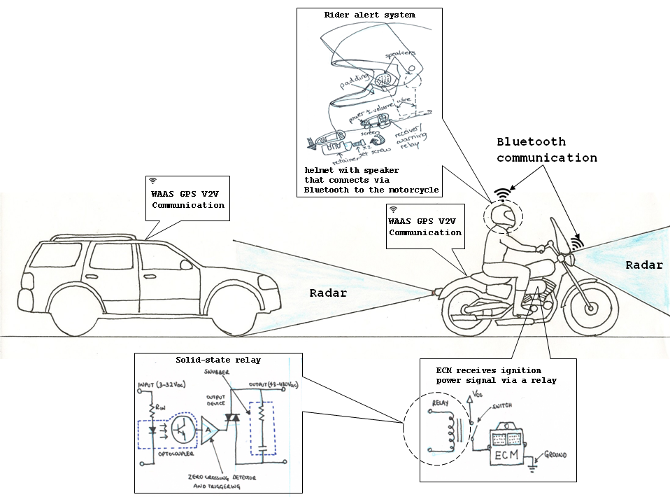
\includegraphics[width=12cm]{MAS_system_overview}
\caption{M\-A\-S system overview}
\end{DoxyImage}
 